\subsection{Anwendungsfall Testfahrzeugkonfiguration}\label{subsec:anwendungsfall-testfahrzeugkonfiguration}

Bevor ein neues Fahrzeug in Serie produziert werden kann,
müssen mit Vorserienfahrzeugen eine bestimmte Anzahl von Tests ausgeführt werden,
um die Funktion der einzelnen Komponenten und die allgemeine Produzierbarkeit sicherzustellen.
Dabei hat sich die Anzahl der zu testenden Funktionen in den letzten Jahren signifikant gesteigert.
Da die Herstellung dieser Vorserienfahrzeuge sehr kostenintensiv und die Ausführung der dazugehörigen
Tests sehr zeitaufwendig ist, soll für eine gegebene Anzahl an Tests die Zahl der zu produzierenden
Testfahrzeuge minimiert werden.

Jeder Test gehört dabei einer bestimmten Kategorie an,
die über die Reihenfolge der Ausführung entscheidet.
Crashtests müssen zum Beispiel immer als letzter Test eines
Vorserienautos durchgeführt werden, da diese Teile der
Vorserienfahrzeuge zerstören können und somit die
Ausführung der anderen Tests unmöglich machen.

Die genauen Zusammenhänge der Testkategorien können den
\cref{fig:test_category,fig:test_category2} entnommen werden.

\begin{figure}[H]
    \centering
    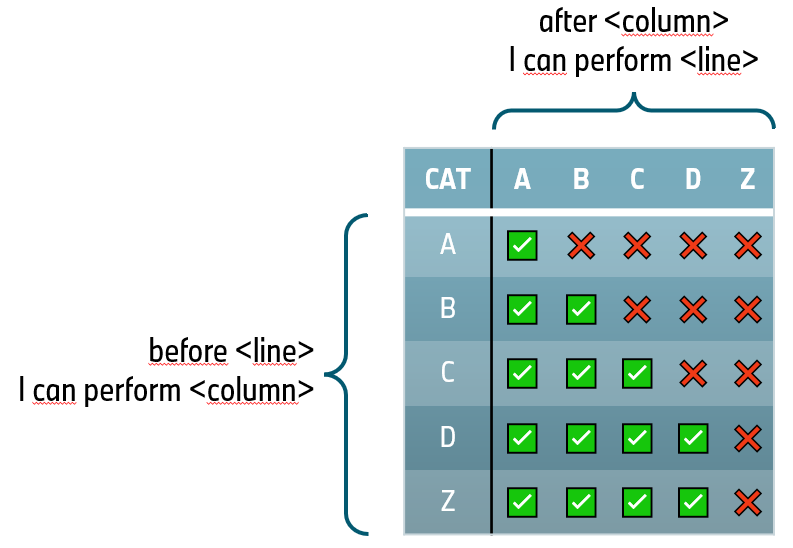
\includegraphics[width=0.6\textwidth]{images/testfahrzeug_problem/Bench-QC_TVC_simplified_Matrix}
    \caption{Zusammenhang der Testkategorien als Matrix}
    \label{fig:test_category}
\end{figure}
\begin{figure}[H]
    \centering
    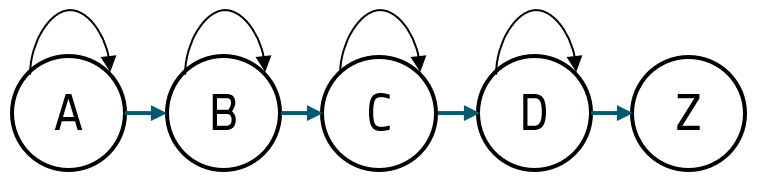
\includegraphics[width=0.6\textwidth]{images/testfahrzeug_problem/Bench-QC_TVC_simplified_dependencies}
    \caption{Zusammenhang der Testkategorien vereinfacht als gerichteter Graph}
    \label{fig:test_category2}
\end{figure}

Die Testfahrzeuge werden in drei verschiedenen, teilweise überlappenden,
Bauphasen produziert, die in \cref{fig:test_times} dargestellt sind.
Jeder Test ist an Fahrzeuge einer bestimmten Bauphase gekoppelt.
Eine Bauphase erstreckt sich über mehr als ein Jahr.
Die Tests müssen spätestens ein Jahr nach Bau eines
Fahrzeugs absolviert sein.
\begin{figure}[H]
    \centering
    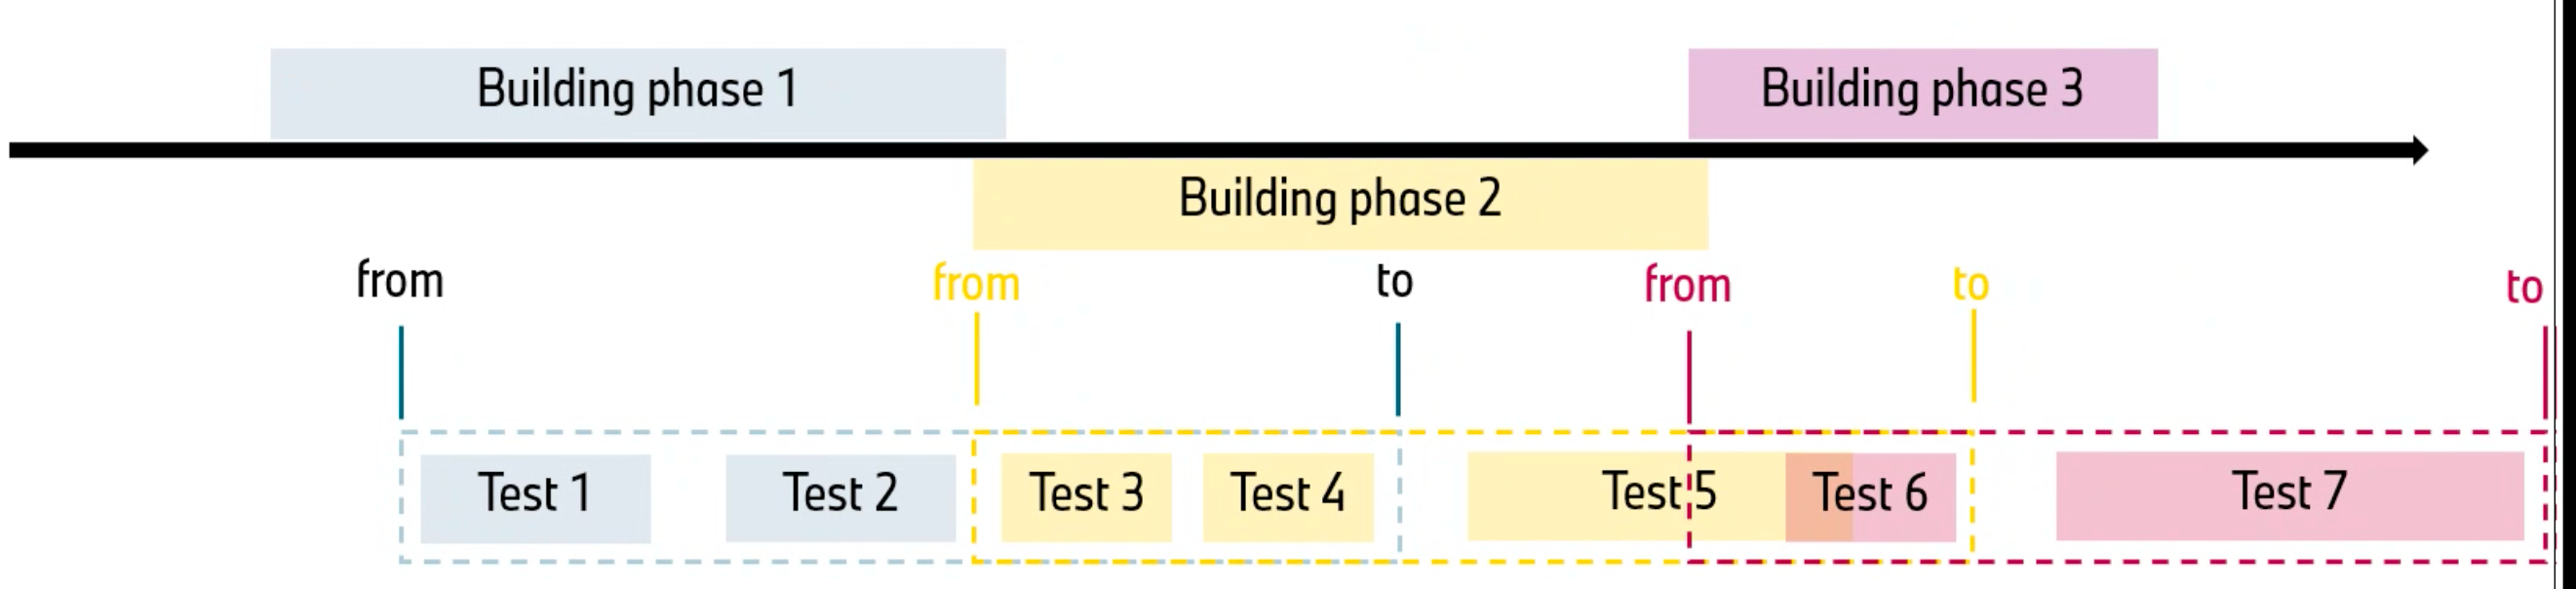
\includegraphics[width=0.9\textwidth]{images/testfahrzeug_problem/test_times}
    \caption{Bauphasen der Vorserienfahrzeuge}
    \label{fig:test_times}
\end{figure}

Pro konkrete Bauphase ist somit eine Menge an Tests vorgegeben,
die auf $n$ verschiedenen Testfahrzeugen durchgeführt werden müssen.
Pro Test sind dabei gewisse Sonderausstattungen (SAs) vorgegeben oder ausgeschlossen.
In Testfahrzeuge können je nach Modelltyp unterschiedliche Sonderausstattungen
verbaut werden. Sonderausstattungen können andere Sonderausstattungen fordern
oder ausschließen. Zum Beispiel kann ein Auto nicht gleichzeitig einen $4$- und $8$
Zylindermotor verbaut haben. Diese direkten Abhängigkeiten können auf die Tests
übertragen werden, so dass eine minimale Anzahl an Testfahrzeugen gefunden werden kann.

\subsubsection{Transformation Testinkompatibilitäten}

Ziel ist es herauszufinden, welche Tests auf demselben Testfahrzeug getestet
werden dürfen. Dies ergibt sich aus den folgenden Informationen:

\begin{itemize}
    \item Abhängigkeiten und Ausschlüsse der SAs
    \item Verfügbare Testfahrzeugkategorien
    \item Forderung von unterschiedlichen Testfahrzeugen
    \item Zugehörigkeit zu Testkategorien
\end{itemize}

\paragraph{Abhängigkeiten und Ausschlüsse der SAs}
Für jeden Tests sollte bekannt sein, welche Sonderausstattung des Testfahrzeugs
gefordert werden sollte. Neben den direkten Abhängigkeiten gibt es auch die
indirekten, die sich aus den geforderten SAs ergeben. Wie die indirekten
Abhängigkeiten auf die Tests übertragen werden können, sollen exemplarisch die
nachfolgenden Regeln zeigen. Angenommen eine Sonderausstattung $SA1$ wird gefordert.

\begin{table}[H]
    \label{tab:tableSAs}
    \begin{tabularx}{\textwidth}{ | l | X |}
        Bedingung an SAs & Abhängigkeit im Test \\\hline\hline
        $SA1 \Rightarrow SA2$ & $SA2$ für Test benötigt \\\hline
        $SA1 \Rightarrow \sim SA2$ & $\sim SA2$  für Test benötigt \\\hline
        $SA1 \Rightarrow SA2~|~SA3$ & $SA2$ oder $SA3$  für Test benötigt \\\hline
        Nur eins $SA1, SA2, SA3$ & $\sim SA2$ und $\sim SA3$  für Test benötigt \\\hline
        $SA1~\&~SA2$ & $SA2$  für Test benötigt \\\hline
        $SA2 \Rightarrow \sim SA1$ & dh. $SA1 \Rightarrow \sim SA2$ \\& $\sim SA2$  für Test benötigt\\\hline
    \end{tabularx}
\end{table}
\todo{Liste ist nicht vollständig!}
Wenn eine benötigte $SA$ oder ausgeschlossene $~SA$ gefunden wurde,
müssen auch für diese die Regeln überprüft werden.

Am Ende ergibt sich eine Menge an Tests, für die bekannt ist,
welche SAs auf dem Testfahrzeug sein müssen und welche SAs nicht erlaubt sind.

Tests, die sich ausschließende SAs haben, können somit nicht auf demselben
Testfahrzeug getestet werden.

\paragraph{Verfügbare Testfahrzeugkategorien}
Des Weiteren sind auch die SAs auf den Testfahrzeugen eingeschränkt.
Testfahrzeuge gehören unterschiedlichen Testfahrzeugkategorien an.
Jede Testfahrzeugkategorie hat erlaubte SAs.
Ein Test kann nur dann durchgeführt werden, wenn mindestens ein Testfahrzeugkategorie
alle benötigten Sonderausstattungen erlaubt. Andernfalls kann dieser Test nicht
ausgeführt werden und die Verteilung aller Tests ist nicht möglich.

Tests, die nicht auf demselben Testfahrzeug ausgeführt werden können,
können ebenfalls gegenseitig ausgeschlossen werden.

\paragraph{Forderung von unterschiedlichen Testfahrzeugen}
Normalerweise müssen Tests mehr als einmal auf unterschiedlichen Testfahrzeugen
durchgeführt werden. Diese Tests schließen sich somit auch gegenseitig aus.

\paragraph{Zugehörigkeit zu Testkategorien}

Aus den Testfahrzeugkategorien ergibt sich die Ausführungsreihenfolge der Tests.
Tests, die zur Kategorie `Z` gehören, dürfen allerdings nur einmal pro Fahrzeug existieren.
Diese Tests sind somit gegenseitig auszuschließen, damit gewährleistet werden kann,
dass nur ein Test pro Fahrzeug zugeteilt werden kann.
Tests anderer Kategorien müssen nicht besonders behandelt werden.

\subsubsection{Transformation zu Bin Packing mit Konflikten}

Gegeben ist eine Liste an Tests einer konkreten Bauphase, die genau einmal durchgeführt werden müssen.
Für jeden Test ist bekannt:
\begin{itemize}
    \item welche Tests nicht am selben Fahrzeug durchgeführt werden dürfen,
    \item wie lange für die Durchführung benötigt wird,
    \item wann er frühestmöglich ausgeführt werden darf und
    \item bis wann er spätestens ausgeführt werden muss.
\end{itemize}

Um die Kosten möglichst gering zu halten, soll die Anzahl der Testfahrzeuge minimal gehalten werden.
Alle Tests müssen ausgeführt werden.

%\subsubsection{Klassische Lösung}\todo[inline]{evtl. ein eigenes Kapitel für das Mapping einfügen.}
Das Testfahrzeugkonfigurationsproblem lässt sich auf das spezielle Bin Packing Problem mit Konflikten
(siehe~\cref{subsubsec:bin-packing-with-conflicts}) abbilden.

Die Testfahrzeuge sind dabei die Behälter, deren Anzahl im Optimum möglichst gering sein muss.
Die Objekte sind die auszuführenden Tests, die in dieser Bauphase abgeschlossen sein müssen.
Die Test-Durchführungszeit ist im klassischen Problem das Gewicht der Objekte.
Die maximale Kapazität pro Testfahrzeug ist ein Jahr, da alle Tests nacheinander ausgeführt werden müssen.

Die letzten beiden Eigenschaften der Tests bezüglich der Ausführungszeit ignorieren wir zunächst.

Zusammengefasst, lässt sich die Testfahrzeugkonfiguration wie folgt auf die Notation aus
\cref{subsubsec:bin-packing-with-conflicts} mappen:
\begin{table}[H]
    \begin{tabularx}{\textwidth}{  l | X | l }
    Symbol & Bedeutung & Definitionsbereich \\\hline\hline
    Mengen & & \\\hline\hline
    $O$ & Menge der Tests & $\N$\\\hline
    $B$ & Menge der Testfahrzeuge & $\N$\\\hline
    $I$ & Menge der inkompatiblen Tests & $\N\times\N$\\\hline\hline
    Konstanten &  &  \\\hline\hline
    $c$ & Ein Jahr & $\N$\\\hline
    $w_o$ & Benötigte Zeit für Test $o\in O$ & $\N$\\\hline\hline
    Variablen &  &  \\\hline\hline
    $x_{ob}$ & Genau dann, wenn $x_{ob}=1$ wird Test $o\in O$ dem Testfahrzeug $b\in B$ zugeteilt & $\B$\\\hline
    \end{tabularx}
    \caption{Notation zu Testfahrzeugkonfiguration}\label{tab:notation_test_vehicle}
\end{table}